% Options for packages loaded elsewhere
\PassOptionsToPackage{unicode}{hyperref}
\PassOptionsToPackage{hyphens}{url}
\PassOptionsToPackage{dvipsnames,svgnames*,x11names*}{xcolor}
%
\documentclass[
  10pt,
  dvipsnames,enabledeprecatedfontcommands]{scrartcl}
\usepackage{amsmath,amssymb}
\usepackage{lmodern}
\usepackage{ifxetex,ifluatex}
\ifnum 0\ifxetex 1\fi\ifluatex 1\fi=0 % if pdftex
  \usepackage[T1]{fontenc}
  \usepackage[utf8]{inputenc}
  \usepackage{textcomp} % provide euro and other symbols
\else % if luatex or xetex
  \usepackage{unicode-math}
  \defaultfontfeatures{Scale=MatchLowercase}
  \defaultfontfeatures[\rmfamily]{Ligatures=TeX,Scale=1}
\fi
% Use upquote if available, for straight quotes in verbatim environments
\IfFileExists{upquote.sty}{\usepackage{upquote}}{}
\IfFileExists{microtype.sty}{% use microtype if available
  \usepackage[]{microtype}
  \UseMicrotypeSet[protrusion]{basicmath} % disable protrusion for tt fonts
}{}
\usepackage{xcolor}
\IfFileExists{xurl.sty}{\usepackage{xurl}}{} % add URL line breaks if available
\IfFileExists{bookmark.sty}{\usepackage{bookmark}}{\usepackage{hyperref}}
\hypersetup{
  pdftitle={Appendix to `The Difficulty with Conjuction': Proofs and Simulations},
  pdfauthor={Marcello Di Bello and Rafal Urbaniak},
  colorlinks=true,
  linkcolor=Maroon,
  filecolor=Maroon,
  citecolor=Blue,
  urlcolor=blue,
  pdfcreator={LaTeX via pandoc}}
\urlstyle{same} % disable monospaced font for URLs
\usepackage{graphicx}
\makeatletter
\def\maxwidth{\ifdim\Gin@nat@width>\linewidth\linewidth\else\Gin@nat@width\fi}
\def\maxheight{\ifdim\Gin@nat@height>\textheight\textheight\else\Gin@nat@height\fi}
\makeatother
% Scale images if necessary, so that they will not overflow the page
% margins by default, and it is still possible to overwrite the defaults
% using explicit options in \includegraphics[width, height, ...]{}
\setkeys{Gin}{width=\maxwidth,height=\maxheight,keepaspectratio}
% Set default figure placement to htbp
\makeatletter
\def\fps@figure{htbp}
\makeatother
\setlength{\emergencystretch}{3em} % prevent overfull lines
\providecommand{\tightlist}{%
  \setlength{\itemsep}{0pt}\setlength{\parskip}{0pt}}
\setcounter{secnumdepth}{5}
%\documentclass{article}

% %packages
\usepackage{booktabs}
%\usepackage[left]{showlabels}
\usepackage{multirow}
\usepackage{subcaption}
\usepackage{wrapfig}
\usepackage{graphicx}
\usepackage{longtable}
\usepackage{ragged2e}
\usepackage{etex}
%\usepackage{yfonts}
\usepackage{marvosym}
\usepackage[notextcomp]{kpfonts}
\usepackage{nicefrac}
\newcommand*{\QED}{\hfill \footnotesize {\sc Q.e.d.}}
\usepackage{floatrow}
\usepackage{multicol}

\usepackage[textsize=footnotesize]{todonotes}
\newcommand{\ali}[1]{\todo[color=gray!40]{\textbf{Alicja:} #1}}
\newcommand{\mar}[1]{\todo[color=blue!40]{#1}}
\newcommand{\raf}[1]{\todo[color=olive!40]{#1}}

%\linespread{1.5}
\newcommand{\indep}{\!\perp \!\!\! \perp\!}


\setlength{\parindent}{10pt}
\setlength{\parskip}{1pt}


%language
%\usepackage{times}
\usepackage{mathptmx}
\usepackage[scaled=0.86]{helvet}
\usepackage{t1enc}
%\usepackage[utf8x]{inputenc}
%\usepackage[polish]{babel}
%\usepackage{polski}




%AMS
\usepackage{amsfonts}
\usepackage{amssymb}
\usepackage{amsthm}
\usepackage{amsmath}
\usepackage{mathtools}

\usepackage{geometry}
 \geometry{a4paper,left=35mm,top=20mm,}


%environments
\newtheorem{fact}{Fact}


% allow page breaks in equations
\allowdisplaybreaks


%abbreviations
\newcommand{\ra}{\rangle}
\newcommand{\la}{\langle}
\newcommand{\n}{\neg}
\newcommand{\et}{\wedge}
\newcommand{\jt}{\rightarrow}
\newcommand{\ko}[1]{\forall  #1\,}
\newcommand{\ro}{\leftrightarrow}
\newcommand{\exi}[1]{\exists\, {_{#1}}}
\newcommand{\pr}[1]{\ensuremath{\mathsf{P}(#1)}}
\newcommand{\cost}{\mathsf{cost}}
\newcommand{\benefit}{\mathsf{benefit}}
\newcommand{\ut}{\mathsf{ut}}

\newcommand{\odds}{\mathsf{Odds}}
\newcommand{\ind}{\mathsf{Ind}}
\newcommand{\nf}[2]{\nicefrac{#1\,}{#2}}
\newcommand{\R}[1]{\texttt{#1}}
\newcommand{\prr}[1]{\mbox{$\mathtt{P}_{prior}(#1)$}}
\newcommand{\prp}[1]{\mbox{$\mathtt{P}_{posterior}(#1)$}}



\newtheorem{q}{\color{blue}Question}
\newtheorem{lemma}{Lemma}
\newtheorem{theorem}{Theorem}
\newtheorem{corollary}{Corollary}[fact]


%technical intermezzo
%---------------------

\newcommand{\intermezzoa}{
	\begin{minipage}[c]{13cm}
	\begin{center}\rule{10cm}{0.4pt}



	\tiny{\sc Optional Content Starts}
	
	\vspace{-1mm}
	
	\rule{10cm}{0.4pt}\end{center}
	\end{minipage}\nopagebreak 
	}


\newcommand{\intermezzob}{\nopagebreak 
	\begin{minipage}[c]{13cm}
	\begin{center}\rule{10cm}{0.4pt}

	\tiny{\sc Optional Content Ends}
	
	\vspace{-1mm}
	
	\rule{10cm}{0.4pt}\end{center}
	\end{minipage}
	}
	
	
%--------------------






















\newtheorem*{reply*}{Reply}
\usepackage{enumitem}
\newcommand{\question}[1]{\begin{enumerate}[resume,leftmargin=0cm,labelsep=0cm,align=left]
\item #1
\end{enumerate}}

\usepackage{float}

% \setbeamertemplate{blocks}[rounded][shadow=true]
% \setbeamertemplate{itemize items}[ball]
% \AtBeginPart{}
% \AtBeginSection{}
% \AtBeginSubsection{}
% \AtBeginSubsubsection{}
% \setlength{\emergencystretch}{0em}
% \setlength{\parskip}{0pt}






\usepackage[authoryear]{natbib}

%\bibliographystyle{apalike}



\usepackage{tikz}
\usetikzlibrary{positioning,shapes,arrows}

\usepackage{booktabs}
\usepackage{longtable}
\usepackage{array}
\usepackage{multirow}
\usepackage{wrapfig}
\usepackage{float}
\usepackage{colortbl}
\usepackage{pdflscape}
\usepackage{tabu}
\usepackage{threeparttable}
\usepackage{threeparttablex}
\usepackage[normalem]{ulem}
\usepackage{makecell}
\usepackage{xcolor}
\ifluatex
  \usepackage{selnolig}  % disable illegal ligatures
\fi

\title{Appendix to `The Difficulty with Conjuction': Proofs and
Simulations}
\author{Marcello Di Bello and Rafal Urbaniak}
\date{}

\begin{document}
\maketitle

This appendix briefly describes the formalism of Bayesian networks,
applies it to the difficulty with conjunction and then establishes
several results about \textit{joint} posteriors, Bayes factors and
likelihood ratios. We provide analytic proofs if possible. We rely on
computer simulations whenever analytic proofs become
unmanageable.\footnote{The R code for the simulations, calculations and
  visualizations is available on the book website LINK TO DOCUMENTATION
  TO BE ADDED LATER.} The simulations were conducted as follows. Given a
direct acyclic graph (DAG) of interest (to be defined later), 100,000
random Bayesian networks were generated whose probability measures had
values sampled from the \textsf{Uniform(0,1)} distribution. For each of
these networks, we calculated the relevant posterior probabilities,
Bayes factors, and likelihood ratios.

\hypertarget{bayesian-networks-and-probabilistic-independence}{%
\subsection*{Bayesian networks and probabilistic
independence}\label{bayesian-networks-and-probabilistic-independence}}
\addcontentsline{toc}{subsection}{Bayesian networks and probabilistic
independence}

A Bayesian network consists of a graphical part---a directed acyclic
graph (DAG)---and a probability measure defined over the nodes
(variables) in the graph. A Bayesian network satisfies the Markov
condition. That is, any node is conditionally independent of its
nondescentants (including ancestors), given its parents. If a
probability measure \(\pr{}\) that is defined over the nodes (variables)
in a graph \(\mathsf{G}\) respects the Markov condition, \(\pr{}\) is
said to be compatible with \(\mathsf{G}\). Graph \(\mathsf{G}\) and
measure \(\pr{}\) can then be combined to form a Bayesian network.

The graphical counterpart of probabilistic independence is
\textbf{d-separation}, \(\indep_d\). Two nodes, \(X\) and \(Y\), are
d-separated given a set of nodes
\(\mathsf{Z}\)---\(X\indep_d Y \vert \mathsf{Z}\) --- iff for every
undirected path from \(X\) to \(Y\) there is a node \(Z'\) on the path
such that either (see Figure \ref{fig:connectionsBN}):

\begin{itemize}

\item $Z' \in \mathsf{Z}$ and there is a \textbf{serial} connection, $\rightarrow Z' \rightarrow$, on the path (\textbf{pipe}),
\item  $Z'\in \mathsf{Z}$ and there is a \textbf{diverging} connection, $\leftarrow Z' \rightarrow $, on the path (\textbf{fork}),
\item There is a \textbf{converging} connection $\rightarrow Z' \leftarrow$ on the path (in which case $Z'$ is a \textbf{collider}), and neither $Z'$ nor its descendants are in $\mathsf{Z}$.
\end{itemize}

\vspace{1mm}

\begin{figure}[H]
\hspace{2mm}\begin{subfigure}[!ht]{0.25\textwidth}

\begin{center}
\includegraphics[width=0.75\linewidth]{conjunction-appendix14_files/figure-latex/unnamed-chunk-2-1} \end{center}
\subcaption{\textsf{Serial: Pipe}}
\end{subfigure} 
\hspace{5mm}\scalebox{1}{\begin{subfigure}[!ht]{0.32\textwidth}
\vspace{1mm}

\begin{center}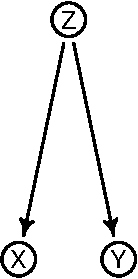
\includegraphics[width=0.75\linewidth]{conjunction-appendix14_files/figure-latex/unnamed-chunk-3-1} \end{center}
\subcaption{\textsf{Diverging: Fork}}
\end{subfigure}}
\hspace{5mm}\scalebox{1}{\begin{subfigure}[!ht]{0.32\textwidth}
\vspace{1mm}

\begin{center}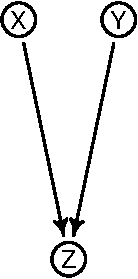
\includegraphics[width=0.75\linewidth]{conjunction-appendix14_files/figure-latex/unnamed-chunk-4-1} \end{center}
\subcaption{\textsf{Converging:Collider}}
\end{subfigure}}
\normalsize
\caption{Three basic types of connections.}
\label{fig:connectionsBN}
\end{figure}

\noindent Serial, converging and diverging connections represent common
scenarios.

Two sets of nodes, \(\mathsf{X}\) and \(\mathsf{Y}\), are d-separated
given \(\mathsf{Z}\) if every node in \(\mathsf{X}\) is d-separated from
every node in \(\mathsf{Y}\) given \(\mathsf{Z}\). Interestingly, it can
be proven that if two sets of nodes are d-separated given a third one,
they are independent given the third one, for any probabilistic measures
compatible with a given DAG. However, lack of d-separation does not
necessarily entail dependence for any probabilistic measure compatible
with a given DAG. It only allows for it: if nodes are d-separated, there
is at least one probabilistic measure fitting the DAG according to which
they are dependent. So, at least, no false independencies can be
inferred from the DAG, and all the dependencies are built into it.

\hypertarget{independencies-in-the-conjunction-problem}{%
\subsection*{Independencies in the conjunction
problem}\label{independencies-in-the-conjunction-problem}}
\addcontentsline{toc}{subsection}{Independencies in the conjunction
problem}

An assumption often made in the formulation of the difficulty with
conjunction is that hypotheses \(A\) and \(B\) are probabilistically
independent. The theory of Bayesian networks helps to formulate this
assumption precisely. The independence of the hypotheses is represented
formally by \textsf{DAG1} in Figure \ref{fig:conjunctionBNs}. The graph
contains nodes for the hypotheses \(A\) and \(B\), the supporting
evidence \(a\) and \(b\), and the conjunctive hypothesis \(A\wedge B\).
The conjunction node \(AB\) is a collider, which guarantees the
independence of \(A\) and \(B\).\footnote{In the Bayesian networks in
  this appendix, the conditional probability table for the conjunction
  node \(AB\) mirrors the truth table for the conjunction in
  propositional logic, as in Table \ref{tab:CPTconjunction2}.} To make
our discussion more general, we will also consider graph \textsf{DAG2}.
This graph relaxes the assumption of independence by drawing an
additional arrow between hypotheses \(A\) and \(B\).

\vspace{1mm}
\footnotesize

\normalsize

\begin{figure}[H]
\hspace{2mm}\scalebox{1}{\begin{subfigure}[!ht]{0.45\textwidth}

\begin{center}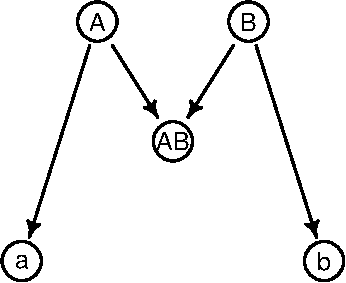
\includegraphics[width=0.75\linewidth]{conjunction-appendix14_files/figure-latex/unnamed-chunk-6-1} \end{center}
\subcaption{\textsf{DAG1}}
\end{subfigure}} 
\hspace{5mm}\begin{subfigure}[!ht]{0.45\textwidth}
\vspace{1mm}

\begin{center}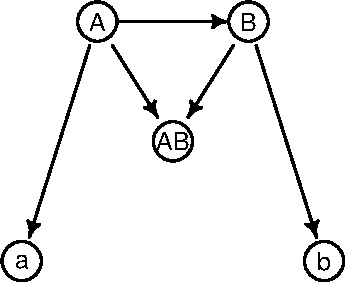
\includegraphics[width=1\linewidth]{conjunction-appendix14_files/figure-latex/unnamed-chunk-7-1} \end{center}
\subcaption{\textsf{DAG2}}
\end{subfigure}
\normalsize
\caption{Two DAGs for the conjunction problem.}
\label{fig:conjunctionBNs}
\end{figure}

\begin{table}[h]
\begin{table}[H]
\centering
\begin{tabular}{lllr}
\toprule
\multicolumn{1}{c}{} & \multicolumn{1}{c}{A} & \multicolumn{1}{c}{B} & \multicolumn{1}{c}{} \\
AB &  &  & Pr\\
\midrule
\cellcolor{gray!6}{1} & \cellcolor{gray!6}{1} & \cellcolor{gray!6}{1} & \cellcolor{gray!6}{1}\\
0 & 1 & 1 & 0\\
\cellcolor{gray!6}{1} & \cellcolor{gray!6}{0} & \cellcolor{gray!6}{1} & \cellcolor{gray!6}{0}\\
0 & 0 & 1 & 1\\
\cellcolor{gray!6}{1} & \cellcolor{gray!6}{1} & \cellcolor{gray!6}{0} & \cellcolor{gray!6}{0}\\
0 & 1 & 0 & 1\\
\cellcolor{gray!6}{1} & \cellcolor{gray!6}{0} & \cellcolor{gray!6}{0} & \cellcolor{gray!6}{0}\\
0 & 0 & 0 & 1\\
\bottomrule
\end{tabular}
\end{table}
\normalsize
\caption{Conditional probability table for the conjunction node.}
\label{tab:CPTconjunction2}
\end{table}

\newpage 
\vspace{1mm}
\footnotesize

\normalsize

Unsurprisingly, the relations of d-separation entailed by the two
networks differ. Examples can be found in Table \ref{tab:indepBNS}. In
fact, \textsf{DAG1} entails 31 d-separations, while \textsf{DAG2}
entails 22 of them. One warning about the notation. Nodes represent
variables, and so each d-separation entails a probabilistic statement
about all combination of the node states (values of variables) involved.
For instance, assuming each node is binary with two possible states, 1
and 0, \mbox{$B   \indep_d\,\,  a $} entails that for any
\mbox{$ B_i, a_i \in \{0, 1\}$} we have
\(\pr{B = B_i} = \pr{B = B_i \vert a = a_i}\).

\begin{table}[h]
\begin{tabular}{cr}
\toprule
Bayesian network 1  & Bayesian network 2\\
\midrule
\cellcolor{gray!6}{$A   \indep_d\,\, B  $}&\cellcolor{gray!6}{     $ A  \indep_d\,\, b \vert  B  $} \\
$A   \indep_d\,\, b  $& $AB  \indep_d\,\,  a \vert  A$\\
\cellcolor{gray!6}{$\,\,\, AB  \indep_d\,\, a \vert A $}  & \cellcolor{gray!6}{$AB  \indep_d\,\,  b \vert  B $}\\
$\,\,\, AB  \indep_d\,\, b \vert B  $ & $ B  \indep_d\,\,  a \vert  A $\\
\cellcolor{gray!6}{$B   \indep_d\,\, a $}        & \cellcolor{gray!6}{$a  \indep_d\,\,  b \vert  B$ }\\
$\,\, a    \indep_d\,\, b$    & $a  \indep_d\,\,  b \vert  A $ \\
\bottomrule
\end{tabular}
\caption{Some of d-separations entailed by \textsf{DAG1} and \textsf{DAG2}.} 
\label{tab:indepBNS}
\end{table}

Turning from nodes to states (or events, propositions), Figure
\ref{tab:indepBNS-states} lists the independencies between
propositions.\footnote{Some caveats. In \eqref{eq:I1} the conditioning
  on \(a\) is not essential, because it's not on the path between the
  nodes: the key reason why the independence remains upon this
  conditioning is that there is an unconditioned collider on the path.
  Still, we need this independence in the proof later on. In
  \eqref{eq:I3} what we are conditioning on is \(A\) and \(B\) jointly.
  Technically, independence conditional on the conjunction node \(AB\)
  does not fall out of the d-separations present in the network---it
  follows given that \(AB\) and \(A,B\) are connected deterministically:
  fixing \(AB\) to true fixes both \(A\) and \(B\) to true.} It also
shows which independencies are entailed by either of the two DAGs.

\begin{figure}
\begin{subfigure}[!ht]{0.45\textwidth}
\begin{align} A\indep B  \label{eq:indAB}     &\hspace{2cm}\mbox{\footnotesize DAG1}\\
b \indep a   \label{eq:indab}   & \hspace{2cm}\mbox{\footnotesize DAG1}\\
A \indep b \vert a   \label{eq:I1}    &\hspace{2cm}\mbox{\footnotesize DAG1} \\
B \indep a \et A \vert b \label{eq:I2}&\hspace{2cm}\mbox{\footnotesize DAG1 } \\
a\indep b \vert A\et B \label{eq:I3}  &\hspace{2cm}\mbox{\footnotesize DAG1 , DAG2} \\  
a\indep b \vert A \label{eq:I3a}   &\hspace{2cm}\mbox{\footnotesize DAG1 , DAG2} \\ 
a\indep b \vert \n A \label{eq:I3b}   &\hspace{2cm}\mbox{\footnotesize DAG1 , DAG2} \\ 
a\indep b \vert B \label{eq:I3a2}   &\hspace{2cm}\mbox{\footnotesize DAG1 , DAG2} \\
a\indep b \vert \n B \label{eq:I3b2}   &\hspace{2cm}\mbox{\footnotesize DAG1 , DAG2}
\end{align}
\end{subfigure}
\begin{subfigure}[!ht]{0.5\textwidth}
\begin{align}
a\indep B \vert A \label{eq:I4}    & \hspace{2cm}\mbox{\footnotesize DAG1 , DAG2} \\
a\indep B \vert \n A \label{eq:I4a}    & \hspace{2cm}\mbox{\footnotesize DAG1 , DAG2} \\
a\indep \n B \vert A \label{eq:I4b}   & \hspace{2cm}\mbox{\footnotesize DAG1 , DAG2} \\
a\indep \n B \vert \n A \label{eq:I4c}   & \hspace{2cm}\mbox{\footnotesize DAG1 , DAG2} \\
b\indep A \et a \vert B \label{eq:I5}  & \hspace{2cm}\mbox{\footnotesize DAG1 , DAG2} \\
b\indep \n A \et a \vert B \label{eq:I5a} &\hspace{2cm}\mbox{\footnotesize DAG1 , DAG2}  \\
b\indep A \et a \vert \n B \label{eq:I5b} & \hspace{2cm}\mbox{\footnotesize DAG1 , DAG2} \\
b\indep \n A \et a \vert \n B \label{eq:I5c} & \hspace{2cm}\mbox{\footnotesize DAG1 , DAG2} \\
b \indep a \vert B \label{eq:I6} & \hspace{2cm}\mbox{\footnotesize DAG1 , DAG2} 
\end{align}
\end{subfigure}
\caption{Independencies among propositions according to \textsf{DAG1} and \textsf{DAG2}.} 
\label{tab:indepBNS-states}
\end{figure}

An ambiguity in our notation is worth mentioning. Table
\ref{tab:indepBNS} lists independencies between \emph{nodes}. But Figure
\ref{tab:indepBNS-states} is about \textit{states} rather than nodes. An
expression such as \mbox{$b\indep A \et a \vert \n B$} should be
understood as a claim about states (events, propositions), which means
the same as
\(\pr{b = 1 \vert B = 0} = \pr{b = 1 \vert A = 1, a = 1, B = 0}\). The
distinction between nodes and their states (or variables and their
values) matters because independence conditional on \(B= 0\) doesn't
entail independence given \(B=1\). For instance, one's final grade might
depend on hard work if the teacher is fair, but this might fail if the
teacher is not fair. We hope this ambiguity in notation will cause no
confusion. Whether we talk about nodes or states (or events,
propositions) should be clear from the context.

\hypertarget{posterior-probabilities}{%
\subsection*{Posterior probabilities}\label{posterior-probabilities}}
\addcontentsline{toc}{subsection}{Posterior probabilities}

We first examine how posterior probabilities behave in the conjunction
problem. The joint posterior \(\pr{A\wedge B \vert a\wedge b}\) is often
lower than the individual posterior \(\pr{A \vert a}\) and
\(\pr{B \vert b}\), whether the hypotheses \(A\) and \(B\) are
independent or not. We establish this fact via a computer simulation. We
simulated 10,000 random Bayesian networks based on \textsf{DAG1}
(independent hypotheses) and \textsf{DAG2} (dependent hypotheses). If
any such network has an equal probability of occurring, the joint
posterior is lower than both individual posteriors 68\% of the time for
\textsf{DAG1}, and around 60\% for \textsf{DAG2}. Figure
\ref{fig:posteriorFailure} displays the distributions of the distances
of the joint posterior from the lowest of the individual posteriors.

\begin{figure}[H]


\begin{center}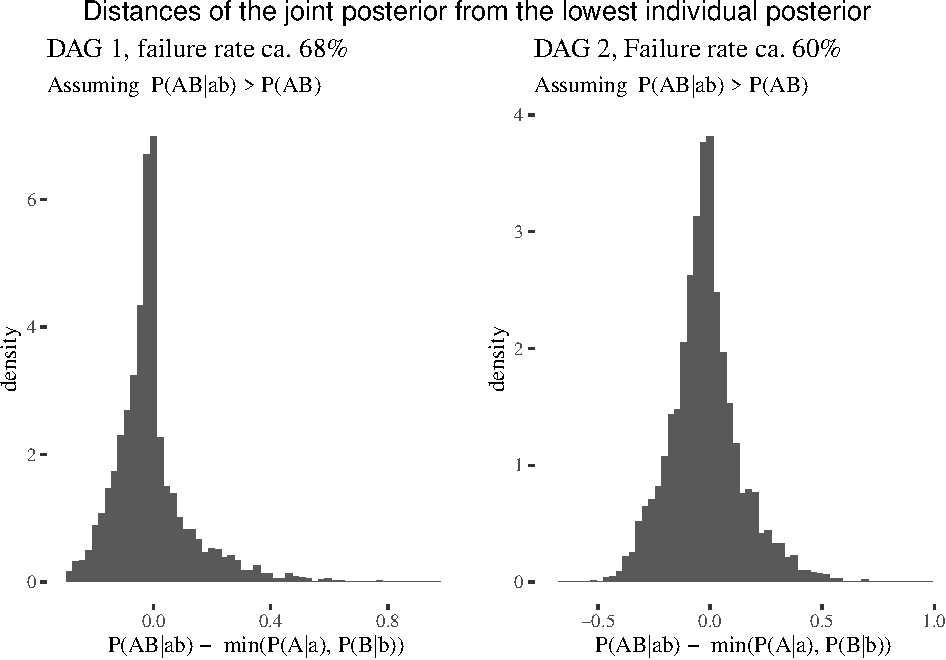
\includegraphics[width=0.75\linewidth]{conjunction-appendix14_files/figure-latex/unnamed-chunk-11-1} \end{center}
\caption{Even assuming the joint support is positive, the joint posterior often is lower than individual posteriors.}
\label{fig:posteriorFailure}
\end{figure}

\hypertarget{bayes-factor-proofs}{%
\subsection*{Bayes factor: proofs}\label{bayes-factor-proofs}}
\addcontentsline{toc}{subsection}{Bayes factor: proofs}

Next, we turn to the Bayes factor. For ease of reference, we use the
following abbreviations: \begin{align*}
BF_A  & =  \frac{\pr{a \vert A}}{\pr{a}},\\
BF_B & = \frac{\pr{b \vert B}}{\pr{b}},\\\
BF_{AB}  & =  \frac{\pr{a\wedge b \vert A \wedge B}}{\pr{a \wedge b}}
\end{align*}

\noindent The objective here is to study how the combined support
\(BF_{AB}\) compares to the individual supports \(BF_A\) and \(BF_B\).
We prove the following general theorem:

\begin{theorem}
Given a measure $\pr{}$ compatible with \textsf{DAG1}, if both $BF_A$ and $BF_B$ 
are grater than one, then $BF_{AB}\geq \mathsf{max}(BF_{A},BF_{B})$.
The same holds for a measure compatible with \textsf{DAG2}.
\label{thm:aggregationBf}
\end{theorem}

\noindent In other words, the combined support \(BF_{AB}\) is never
below the individual supports \(BF_A\) and \(BF_B\), whether claims
\(A\) and \(B\) are independent (\textsf{DAG1}) or not (\textsf{DAG2}).

\begin{proof}
For \textsf{DAG1}, the theorem holds by Fact \ref{fac:BFindep} (and corollary). For 
\textsf{DAG2}, the theorem holds by Fact \ref{fac:BFdep} (and corollary), Lemma \ref{lem:BFLR}, and Fact \ref{fact:BFweaker3}. 
\end{proof}

\begin{fact} If the independence assumptions \eqref{eq:indAB}, \eqref{eq:indab}, \eqref{eq:I4} and \eqref{eq:I5} hold (all of which are entailed by \textsf{DAG1}), then 
$BF_{AB} = BF_A \times BF_B$. \label{fac:BFindep}
\end{fact}

\begin{proof}

\begin{align*}
\frac{\pr{a \wedge b\vert A\wedge B}}{\pr{a \wedge b}} & = \frac{\pr{A \et B\et a\wedge b}}{\pr{A \et B}} \bigg/ \pr{a \wedge b}
&\mbox{(conditional probability)} \\
&  = \frac{\pr{A} \times \pr {B \vert A}  \times \pr{a \vert A \et B} \times \pr{b \vert A \et B \et a}}{\pr{A \et B}} \bigg/ \pr{a \wedge b}
&\mbox{\,\,\,\,\,\,\, (chain rule)} \\
\end{align*}

\noindent Next, we apply the relevant independence assumptions:

\begin{align*}
&  = \frac{\pr{A} \times \overbrace{\pr {B \vert A}}^{ \pr{B} \mbox{\footnotesize \, by \eqref{eq:indAB}}}  \times
\overbrace{\pr{a \vert A \et B}}^{\pr{a \vert A} \mbox{\footnotesize \, by \eqref{eq:I4}}}
\times \overbrace{\pr{b \vert A \et B \et a}}^{\pr{b \vert B} \mbox{\footnotesize \, by \eqref{eq:I5}}}
}{\underbrace{\pr{A \et B}}_{\pr{A} \times \pr{B} \mbox{\footnotesize \, by \eqref{eq:indAB}}}} \bigg/ \underbrace{\pr{a \wedge b}}_{\pr{a}\times \pr{b} \mbox{ \footnotesize \, by \eqref{eq:indab}}} \\
&  = \frac{\pr{A} \times  \pr{B}   \times \pr{a \vert A}  \times  \pr{b \vert B}}
{\pr{A} \times \pr{B}} \bigg/ \pr{a}\times \pr{b} \\
& = \frac{\pr{a \vert A}  }{\pr{a}}  \times \frac{\pr{b \vert B}}{\pr{b}} \\
& = BF_{A} \times BF_B
\end{align*}

\end{proof}

This fact has the following straightforward consequences. They hold
because, if \(a = b \times c\) and \(b, c>1\), then
\(a > \mathsf{max}(b,c)\), and if \(b, c<1\), then
\(a < \mathsf{min}(b,c)\).

\begin{corollary} If the independence assumptions \eqref{eq:indAB}, \eqref{eq:indab}, \eqref{eq:I4} and \eqref{eq:I5} hold, and $BF_{A}$ and $BF_{B}$ are both greater than 1, then $BF_{AB}$ is greater than one. In fact,  $BF_{AB}$ is  greater than  $\mathsf{max}(BF_{A},BF_{B})$. \label{cor:BFind2}
\end{corollary}

\begin{corollary} If the independence assumptions \eqref{eq:indAB}, \eqref{eq:indab}, \eqref{eq:I4} and \eqref{eq:I5} hold, and $BF_{A}$ and $BF_{B}$ are both strictly less than 1, then $BF_{AB}$  is less than  $\mathsf{min}(BF_{A}, BF_{B})$. \label{cor:BFind3}
\end{corollary}

This establishes Theorem \ref{thm:aggregationBf} for \textsf{DAG 1}.
After dropping the independence assumptions specific to \textsf{DAG1}
and shifting to \textsf{DAG 2}, the combined \(BF_{AB}\) can no longer
be obtained by multiplying the individual ones, although multiplication
still provides a decent approximation (see Figure \ref{fig:BFmulti}).

\begin{figure}[H]

\begin{center}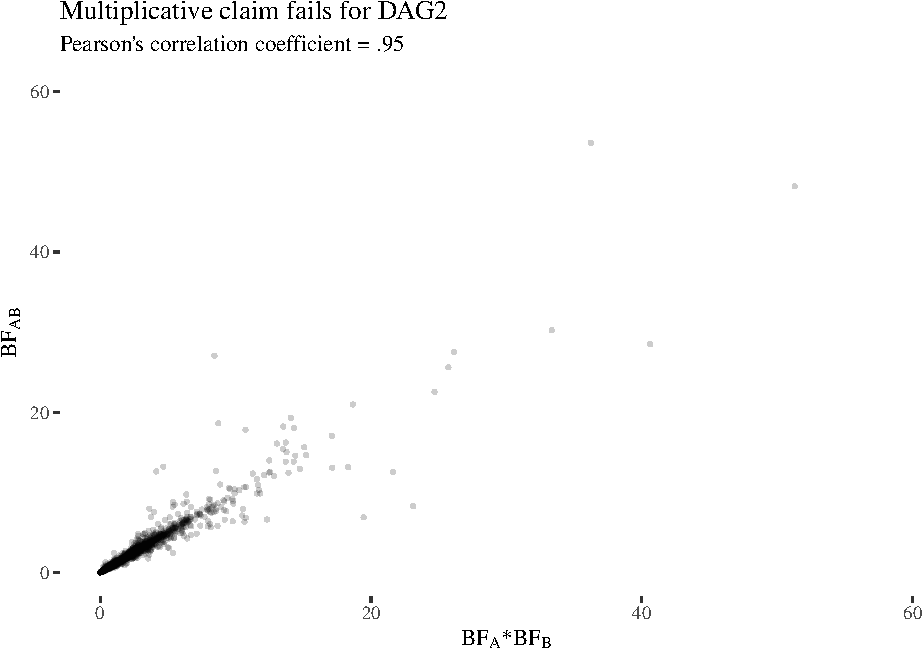
\includegraphics[width=0.75\linewidth]{conjunction-appendix14_files/figure-latex/unnamed-chunk-12-1} \end{center}
\caption{In DAG2, the result of multiplying individual BFs does not equal the joint BF, but often is a good approximation thereof. Axes restricted to $0,60$ (one extreme outlier lying close to the diagonal dropped).}
\label{fig:BFmulti}
\end{figure}

However, if the probabilistic measure fits \textsf{DAG 2}, Theorem
\ref{thm:aggregationBf} is still satisfied. First, we abbreviate:
\begin{align*}
BF^{'}_{B} & = \frac{\pr{b \vert B}}{\pr{b\vert a}} \\
BF^{'}_{A} & = \frac{\pr{a \vert A}}{\pr{a \vert b}}
\end{align*} \noindent A claim weaker than Fact \ref{fac:BFindep} can be
proven by relying only on the independencies entailed by \textsf{DAG2}.

\begin{fact} If \eqref{eq:I4} and \eqref{eq:I5}  hold (and they do in BNs based on \textsf{DAG 2}), then $BF_{AB} =  BF_{A}\times BF^{'}_{B}  = BF_{B} \times BF^{'}_{A}$. \label{fac:BFdep}
\end{fact}

\begin{proof}

We start with the definition of conditional probability and the chain rule, as in the proof of Fact \ref{fac:BFindep}, but now we use fewer independencies (all of them entailed by \textsf{DAG2}). 

 \begin{align*}
\frac{\pr{a \wedge b\vert A\wedge B}}{\pr{a \wedge b}} &
= \frac{\pr{A} \times \pr {B \vert A}  \times
\overbrace{\pr{a \vert A \et B}}^{\pr{a \vert A} \mbox{\footnotesize \, by \eqref{eq:I4}}}
\times \overbrace{\pr{b \vert A \et B \et a}}^{\pr{b \vert B} \mbox{\footnotesize \, by \eqref{eq:I5}}}
}{\underbrace{\pr{A \et B}}_{\pr{A} \times \pr{B\vert A} \mbox{\footnotesize \, by the chain rule}}} \bigg/ \underbrace{\pr{a \wedge b}}_{\pr{a}\times \pr{b\vert a} \mbox{ \footnotesize \, by the chain rule }}\\
& = \frac{\pr{a \vert A}}{\pr{a}} \times \frac{\pr{b\vert B}}{\pr{b \vert a}}\\
& = BF_{A} \times BF^{'}_{B}
\end{align*}
If, instead of obtaining $\pr{a}\pr{b \vert a}$ in the denominator, we deploy the chain rule differently, resulting in $\pr{b}\pr{a \vert b}$, we end up with:
\begin{align*}
& = \frac{\pr{a \vert A}}{\pr{a \vert b}} \times \frac{\pr{b\vert B}}{\pr{b}}\\
& = BF^{'}_{A} \times BF_{B}
\end{align*}

\end{proof}

\begin{corollary} Suppose \eqref{eq:I4} and \eqref{eq:I5}  hold (they are entailed by \textsf{DAG 2}), and $BF_{BA}, BF_{B} >1$. Then if both $\pr{a\vert b} \leq \pr{a \vert A}$ and  $\pr{b \vert a} \leq \pr{b\vert B}$, we have $BF_{AB}\geq BF_{A}, BF_{B}$. \label{cor:BFweaker2}
\end{corollary}

\begin{proof}
Assume the first conjunct holds. Then $\frac{\pr{a\vert A}}{\pr{a\vert b}} \geq 1$ and so:
\begin{align*}
BF_{AB} &= BF^{'}_{A} \times BF_{B} \geq BF_{B}
\end{align*}
\noindent The argument for the other comparison is analogous.
\end{proof}

The proof of Theorem \ref{thm:aggregationBf} for \textsf{DAG 2} is not
complete yet. This corollary relies on the additional assumptions
\(\pr{a\vert b} \leq \pr{a \vert A}\) and
\(\pr{b \vert a} \leq \pr{b\vert B}\). They seem plausible. If, say,
\(a\) is used as evidence for \(A\), we often expect \(A\) and \(a\) to
be fairly strongly connected, that is, we expect \(\pr{a\vert A}\) to be
rather high, while the connection between different pieces of evidence
for different hypotheses, intuitively, is not expected to be as strong.
We provide a proof of these assumptions below.

We start with the following lemma.

\begin{lemma} For any probabilistic measure $\mathsf{P}$, if $BF_A >1$, then $LR_A>1$.\label{lem:BFLR}
\end{lemma}

\begin{proof} We start with our assumption.


\begin{align*}
1 & \leq \frac{\pr{a \vert A}}{\pr{a}} & &  \,\, (BF_A \geq 1) \\
\pr{A} & \leq  \frac{\pr{a \vert A}}{\pr{a}} \pr{A} & & (\mbox{algebraic manipulation}) \\
\pr{A} & \leq \pr{A \vert a} & &  (\mbox{Bayes' theorem})  \\
- \pr{A} &\geq - \pr{A \vert a} &  &   (\mbox{algebraic manipulation}) \\
1- \pr{A} & \geq 1 - \pr{A \vert a} & & (\mbox{algebraic manipulation})\\
1- \pr{A}  & \geq \pr{\n A \vert a} & & (\mbox{algebraic manipulation})\\
\pr{a}\left( 1 - \pr{A}\right) & \geq \pr{a}\pr{\n A \vert a}  & & (\mbox{algebraic manipulation})\\
\pr{a} & \geq \frac{\pr{a} \pr{\n A \vert a}}{\pr{\n A}} &  & (\mbox{algebraic manipulation, negation}) \\
\pr{a} & \geq \pr{a \vert \n A}  & &   (\mbox{conditional probability}) \\
\end{align*}
From this and our assumption  that $\pr{a \vert A} \geq \pr{a}$ it follows that $\pr{a \vert A}\geq \pr{a \vert \n A}$, that is, that \mbox{$LR_A \geq 1$}.
\end{proof}

Now the main claim.

\begin{fact}
For any probabilistic measure $\mathsf{P}$ appropriate for \textsf{DAG 2}, if $BF_A >1$, then $\pr{a \vert A} \geq \pr{a \vert b}$ and 
$\pr{b \vert B} \geq \pr{b \vert a}$.
\label{fact:BFweaker3}
\end{fact}

\begin{proof}

Let's focus on the first conjunct. First, we have:
\begin{align*}
\pr{a \vert b} & = \pr{a \et A \vert b} + \pr{a \et \n A \vert b} & &   (\mbox{total probability}) \\
& = \underbrace{\pr{a \vert b \et A}}_{\pr{a \vert A}  \mbox{\footnotesize \, by \eqref{eq:I3a}}} \pr{A \vert b} +
\underbrace{\pr{a \vert b \et \n A}}_{\pr{a \vert \n A} \mbox{\footnotesize \, by \eqref{eq:I3b}}}\pr{\n A \vert b}  & &   (\mbox{chain rule}) \\
\end{align*}

Now let's introduce some abbreviations:
\begin{align*}
& = \underbrace{\pr{a\vert A}}_k \underbrace{\pr{A \vert b}}_x + \underbrace{\pr{a \vert \n A}}_t \underbrace{\pr{\n A \vert b}}_{(1- x)}
\end{align*}

\noindent Note that the assumption that $BF_A\geq 1$ entails, by Lemma \ref{lem:BFLR}, that $k \geq t$, and so $k-t \geq 0$. Also, since $x$ is a probability, we know $0 \leq x \leq 1$. This allows us to reason algebraically as follows:

\begin{align*}
k & \geq k  \\
k & \geq t + (k - t) \\
k & \geq t + (k -t)x \\
k & \geq kx + t  - tx \\
\pr{a \vert A} = k & \geq kx + t(1-x) = \pr{a \vert b}
\end{align*}

For the second conjunct, notice that we have a similar reasoning, albeit it relies on a different pair of independencies (which nevertheless holds in \textsf{DAG1} and \textsf{DAG 2}).
\begin{align*}
\pr{b \vert a} & = \pr{b \et B \vert a} + \pr{b \et \n B \vert a} & &   (\mbox{total probability}) \\
& = \underbrace{\pr{b \vert a \et B}}_{\pr{b \vert B}  \mbox{\footnotesize \, by \eqref{eq:I3a2}}} \pr{B \vert a} +
\underbrace{\pr{b \vert a \et \n B}}_{\pr{b \vert \n B} \mbox{\footnotesize \, by \eqref{eq:I3b2}}}\pr{\n B \vert a}  & &   (\mbox{chain rule}) \\
\end{align*}

\noindent The rest of the reasoning for this case is algebraically the same as the one used above.
\end{proof}

\hypertarget{bayes-factor-simulations}{%
\subsection*{Bayes factor: simulations}\label{bayes-factor-simulations}}
\addcontentsline{toc}{subsection}{Bayes factor: simulations}

Computer simulations provide additional insights. The joint \(BF_{AB}\)
may be lower than the individual \(BF_A\) and \(BF_B\). Simulated cases
in which \(BF_{AB} < BF_{A}, BF_{B}\) are about 25\% of the total (which
is twice higher than for the likelihood ratio; more on this later). Such
cases are displayed in Figure \ref{fig:BFfails}.

\vspace{1mm}
\footnotesize

\normalsize

\vspace{1mm}
\footnotesize

\normalsize

\begin{figure}

\begin{center}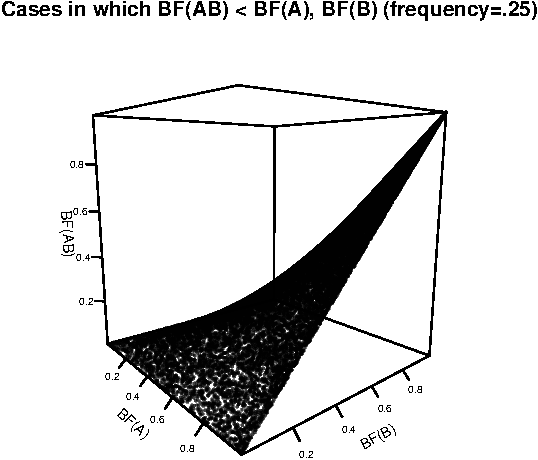
\includegraphics[width=0.7\linewidth]{conjunction-appendix14_files/figure-latex/unnamed-chunk-15-1} \end{center}
\caption{25k cases (out of simulated 100k) in which the joint BF is below each of the individual BFs.}
\label{fig:BFfails}
\end{figure}

This result is nothing surprising. It happens when \(BF_A\) and \(BF_B\)
are lower than one. When they are greater than one, the joint
\(BF_{AB}\) exceeds the individual ones. The distribution of Bayes
factors based on \textsf{DAG1} and \textsf{DAG2} are displayed in Figure
\ref{fig:DAG1BF} and Figure \ref{fig:BFind2}. The distribution is
unchanged in the two cases.

These simulations and the earlier theorem demonstrate that, whenever
individual \(BF_A\) and \(BF_B\) are above a fixed threshold, so is the
combined \(BF_{AB}\). This fact justifies the principle of aggregation,
as explained in the main text of the chapter. But the converse does not
hold. Even when \(BF_{AB}\) is above a threshold, \(BF_A\) or \(BF_B\)
may be below the threshold. Such cases for \textsf{DAG1} and
\textsf{DAG2} are displayed in Figure \ref{fig:BFdistr}. Hence, the
converse of aggregation, the principle of distribution, fails.

\begin{figure}

\begin{center}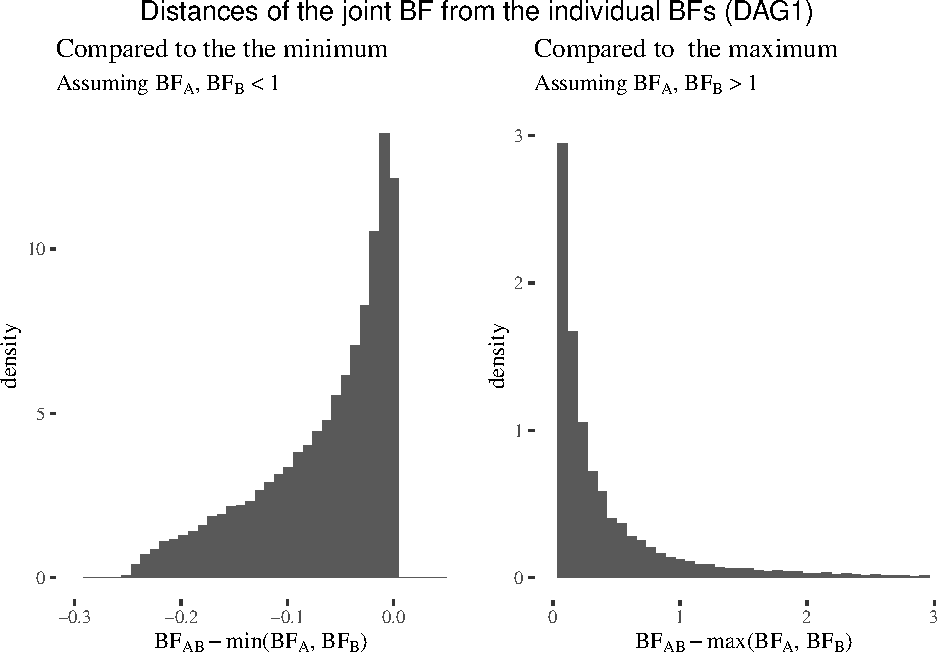
\includegraphics[width=0.7\linewidth]{conjunction-appendix14_files/figure-latex/BFind-1} \end{center}
\caption{Distances of the joint Bayes factor from maxima and minima of individual Bayes factors, depending on whether the individual support levels are both positive or both negative. Simulation based on 100k Bayesian networks build over \textsf{DAG1}.}
\label{fig:DAG1BF}
\end{figure}

\begin{figure}

\begin{center}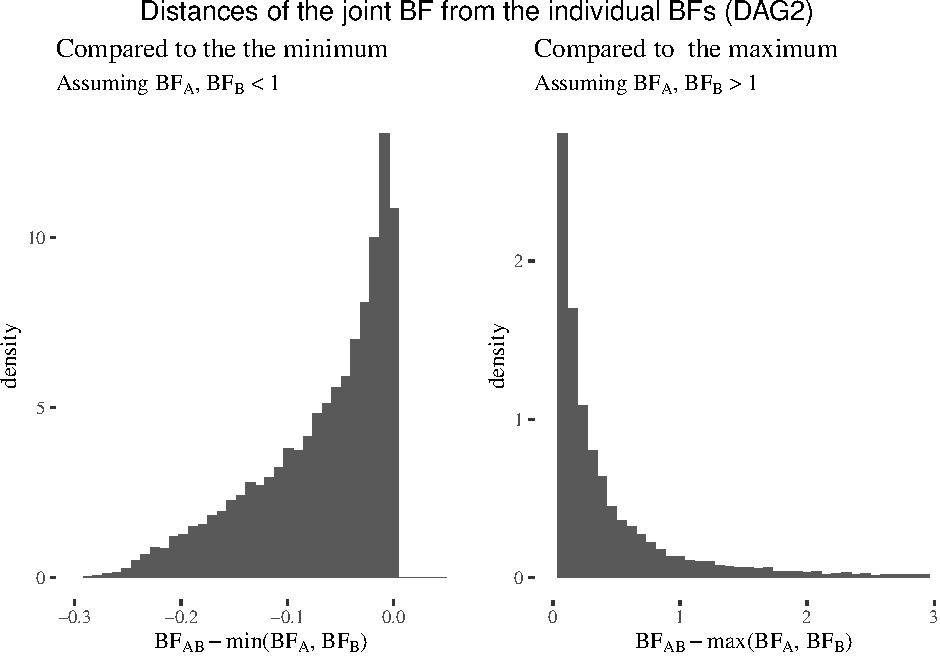
\includegraphics[width=0.7\linewidth]{conjunction-appendix14_files/figure-latex/BFind2-1} \end{center}

\caption{Distances of the joint Bayes factor from maxima and minima of individual Bayes factors, depending on whether the individual support levels are both positive or both negative. Simulation based on 100k Bayesian networks build over \textsf{DAG2}.}
\label{fig:BFind2}
\end{figure}

\vspace{1mm}
\footnotesize

\normalsize

\begin{figure}

\begin{center}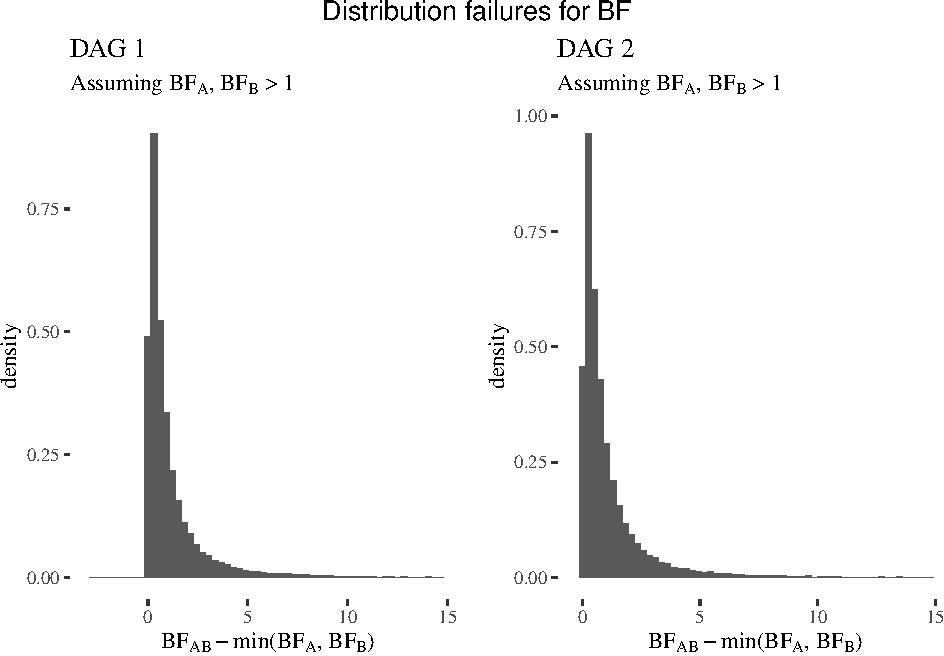
\includegraphics[width=0.7\linewidth]{conjunction-appendix14_files/figure-latex/plotBFDistr-1} \end{center}
\caption{Distribution failure for the Bayes factor, \textsf{DAG 1}. The $x$ axis restricted to $(-3,15)$ for visibility.}
\label{fig:BFdistr}
\end{figure}

\newpage

\hypertarget{likelihood-ratio-proofs}{%
\subsection*{Likelihood ratio: proofs}\label{likelihood-ratio-proofs}}
\addcontentsline{toc}{subsection}{Likelihood ratio: proofs}

We now turn to the likelihood ratio. For ease of reference, we use the
following abbreviations:

\begin{align*}
LR_{AB} &= \frac{\pr{a\wedge b \vert a\wedge B}}{\pr{a \wedge b \vert \neg (A\wedge B)}}\\
LR_A & = \frac{\pr{a \vert A}}{\pr{a \vert \n A}} \\
LR_B & = \frac{\pr{b \vert B}}{\pr{b \vert \n B}}.
\end{align*}

\begin{fact} If independence conditions  \eqref{eq:I4}, \eqref{eq:I4a}, \eqref{eq:I4b},   \eqref{eq:I4c},  \eqref{eq:I5},   \eqref{eq:I5a},    \eqref{eq:I5b}, and   \eqref{eq:I5c}    hold, then:
\begin{align*}
LR_{AB} & =  \frac{\pr{a \vert A} \times \pr{b \vert B}}
 {\frac{\pr{\neg A}\pr{B \vert \neg A} \pr{a \vert \neg A}\pr{b \vert B} + \pr{A}\pr{\neg B \vert A} \pr{a \vert A }\pr{b \vert \neg B} + \pr{\neg A}\pr{\neg B \vert \neg A } \pr{a \vert \neg A}\pr{b \vert \neg B}}{\pr{\neg A}\pr{B \vert \neg A} + \pr{A}\pr{\neg B \vert A } + \pr{\neg A}\pr{\neg B \vert \neg A} }}
\end{align*}
\end{fact}

\noindent Note that these independence assumptions are entailed not only
in \textsf{DAG1}, but also in \textsf{DAG2}.

\begin{proof}
Let's first compute the numerator of $LR_{AB}$:

\begin{align*}
\pr{a \wedge b\vert A\wedge B} & =  \frac{\pr{A \et B \et a\et b}}{\pr{A \et B}}
&\mbox{(conditional probability)}
\\
&= \frac{   \pr{A} \times \pr{B\vert A} \times \pr{a \vert A \wedge B} \times \pr{b \vert A \wedge B \wedge a} }{\pr{A} \times \pr{B \vert A}}
&\mbox{(chain rule)}
\end{align*}

We deploy the relevant independencies as follows:
\begin{align*}
\mbox{      } &= \frac{   \pr{A} \times \pr{B\vert A} \times \overbrace{\pr{a \vert A \wedge B}}^{\pr{a \vert A} \mbox{ \footnotesize \, by \eqref{eq:I4} } } \times \overbrace{\pr{b \vert A \wedge B \wedge a}}^{\pr{b \vert B} \mbox{ \footnotesize \, by \eqref{eq:I5} }} }{\pr{A} \times \pr{B \vert A}}
&\mbox{}\\
 & = \pr{a \vert A} \times \pr{b \vert B} 
 &\mbox{(algebraic manipulation)} 
\end{align*}


\noindent The denominator of $LR_{AB}$ is more complicated, mostly because of the conditioning on  $\neg (A \wedge B)$.

\scalebox{.85}{\parbox{1\linewidth}{
\begin{align*}
\pr{a \et b\vert \neg (A\et B)} & = \frac{\pr{a \et b \et \neg (A\et B)}}{\pr{\neg (A \et B)}} 
&\mbox{ (conditional probability)}\\
& = \frac{\pr{a \et b \et \neg A\et B} +  \pr{a \et b \et A\et \neg B} + \pr{a \et b \et \neg A\et \neg B}  }{\pr{\neg A \et B} + \pr{A \et \neg B} + \pr{\neg A \et \neg B} } 
&\mbox{ (logic \& additivity)}
\end{align*}
}}



\noindent Now consider the first summand from the numerator:
\begin{align*}
\pr{a \et b \et \neg A\et B} & = \pr{\n A} \pr{B \vert \n A} \pr{a \vert \n A \et B} \pr{b\vert a \et \n A \et B} &\mbox{\,\,\,\,\,\,\,\,\,\,\,\,\, (chain rule)} \\ & = 
\pr{\neg A}\pr{B \vert \neg A} \pr{a \vert \neg A}\pr{b \vert B}
&\mbox{\,\,\,\,\,\,\,\,\,\,\,\,\, (independencies \eqref{eq:I4a} and \eqref{eq:I5a})} \\
\end{align*}

The simplification of the other two summanda is analogous (albeit with slightly different independence assumptions---\eqref{eq:I4b} and \eqref{eq:I5b} for the second one and \eqref{eq:I4c} and \eqref{eq:I5c} for the third. Once we plug these into the denominator formula we get:

\scalebox{.8}{\parbox{1\linewidth}{
\begin{align*}
\pr{a \et b\vert \neg (A\et B)} & = \frac{\pr{\neg A}\pr{B \vert \neg A} \pr{a \vert \neg A}\pr{b \vert B} + \pr{A}\pr{\neg B \vert A} \pr{a \vert A }\pr{b \vert \neg B} + \pr{\neg A}\pr{\neg B \vert \neg A } \pr{a \vert \neg A}\pr{b \vert \neg B}}{\pr{\neg A}\pr{B \vert \neg A} + \pr{A}\pr{\neg B \vert A } + \pr{\neg A}\pr{\neg B \vert \neg A} } \\
 & = \frac{\pr{\neg A}\pr{B \vert \neg A} \pr{a \vert \neg A}\pr{b \vert B} + \pr{A}\pr{\neg B \vert A} \pr{a \vert A }\pr{b \vert \neg B} + \pr{\neg A}\pr{\neg B \vert \neg A } \pr{a \vert \neg A}\pr{b \vert \neg B}}{\pr{\neg A}\pr{B \vert \neg A} + \pr{A}\pr{\neg B \vert A } + \pr{\neg A}\pr{\neg B \vert \neg A} }  
 \end{align*}}}

\end{proof}

\hypertarget{likelihod-ratio-simulations}{%
\subsection*{Likelihod ratio:
simulations}\label{likelihod-ratio-simulations}}
\addcontentsline{toc}{subsection}{Likelihod ratio: simulations}

Here the analytic approach is cumbersome. Instead, we mostly rely on
computer simulations. First of all, the joint \(LR_{AB}\) can be lower
than any of the individual \(LR_A\) and \(LR_B\). Based on \textsf{DAG1}
and \textsf{DAG2}, the frequency of such cases in which
\(LR_{AB} < LR_{A}, LR_{B}\) is about 12.5\%, half the frequency for the
Bayes factor. The distribution of these cases is displayed in Figure
\ref{fig:LRfails}.

\begin{figure}

\begin{center}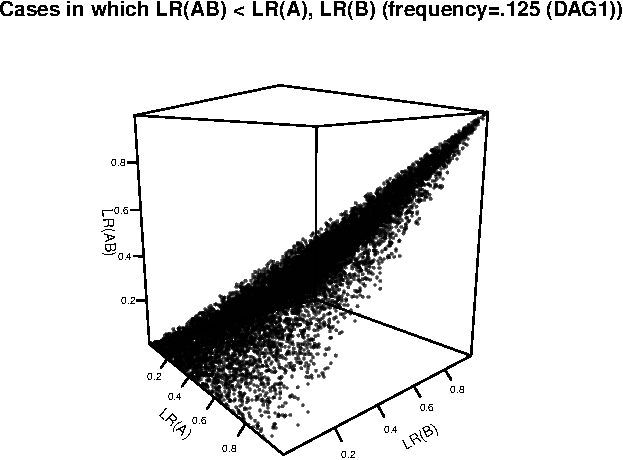
\includegraphics[width=0.6\linewidth]{conjunction-appendix14_files/figure-latex/unnamed-chunk-17-1} \end{center}
\caption{12.5k cases (out of simulated 100k) in which the joint LR is below each of the individual LRs.  The picture for \textsf{DAG2} is very similar.}
\label{fig:LRfails}
\end{figure}

Consider now cases in which both individual likelihood ratios are above
one. Interestingly, one of the individual likelihood ratios, \(LR_A\) or
\(LR_B\), may be greater than the joint \(LR_{AB}\) (see example in
Figure \ref{tab:CPTconjunctionBNL}). This does not happen with the Bayes
factor. But even though the joint likelihood ratio can be lower than the
maximum, it is never lower than the minimum of the individual likelihood
ratios (Figures \ref{fig:LRabovePlot} and \ref{fig:LRabovePlotDep}).
Conversely, if both individual likelihood ratios are below one, the
joint likelihood ratio can be higher than their minimum, but is never
higher than their maximum (Figures \ref{fig:LRlowerPlot} and
\ref{fig:LRlowerPlot2}).

\vspace{1mm}
\footnotesize

\normalsize

\vspace{1mm}
\footnotesize

\normalsize

\begin{figure}
\begin{subfigure}[!ht]{0.45\textwidth}

\footnotesize 
\begin{tabular}{lr}
\toprule
A & Pr\\
\midrule
\cellcolor{gray!6}{1} & \cellcolor{gray!6}{0.892}\\
0 & 0.108\\
\bottomrule
\end{tabular}

\vspace{2mm}

\begin{tabular}{lrr}
\toprule
\multicolumn{1}{c}{B} & \multicolumn{2}{c}{A} \\
  & 1 & 0\\
\midrule
\cellcolor{gray!6}{1} & \cellcolor{gray!6}{0.551} & \cellcolor{gray!6}{0.457}\\
0 & 0.449 & 0.543\\
\bottomrule
\end{tabular}

\vspace{2mm}

\begin{tabular}{lrr}
\toprule
\multicolumn{1}{c}{a} & \multicolumn{2}{c}{A} \\
  & 1 & 0\\
\midrule
\cellcolor{gray!6}{1} & \cellcolor{gray!6}{0.957} & \cellcolor{gray!6}{0.453}\\
0 & 0.043 & 0.547\\
\bottomrule
\end{tabular}


\vspace{2mm}

\begin{tabular}{lrr}
\toprule
\multicolumn{1}{c}{b} & \multicolumn{2}{c}{B} \\
  & 1 & 0\\
\midrule
\cellcolor{gray!6}{1} & \cellcolor{gray!6}{0.678} & \cellcolor{gray!6}{0.573}\\
0 & 0.322 & 0.427\\
\bottomrule
\end{tabular}

\vspace{2mm}

\normalsize
\end{subfigure} \begin{subfigure}[!ht]{0.45\textwidth}

\begin{center}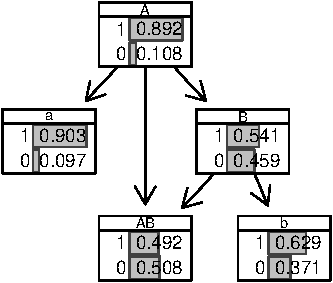
\includegraphics[width=0.7\linewidth]{conjunction-appendix14_files/figure-latex/unnamed-chunk-21-1} \end{center}
\end{subfigure}
\caption{$LR_A  \approx 2.11$, $LR_B \approx 1.183$,  $LR_{AB} \approx 1.319$. \newline  $BF_A \approx  1.06, BF_B \approx  1.076, BF_{AB}\approx   1.14$.}
\label{tab:CPTconjunctionBNL}
\end{figure}

\begin{figure}


\begin{center}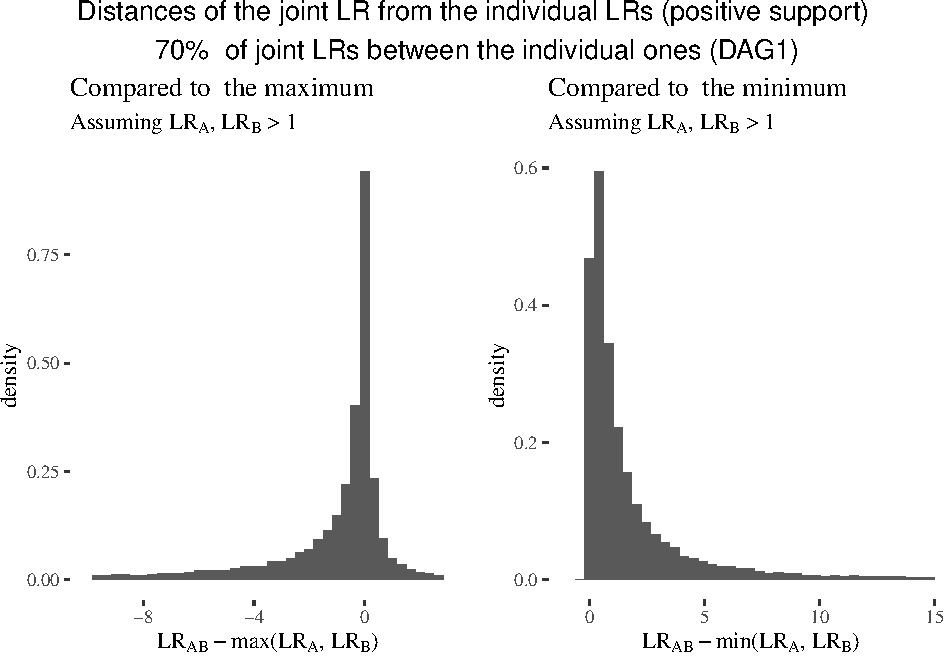
\includegraphics[width=0.7\linewidth]{conjunction-appendix14_files/figure-latex/unnamed-chunk-22-1} \end{center}

\caption{Distances of joint likelihood ratios for the minima and the maxima of the individual likelihood ratios if the individual likelihood ratios are above 1, DAG used in \textsf{DAG1}.}
\label{fig:LRabovePlot}
\end{figure}

\begin{figure}


\begin{center}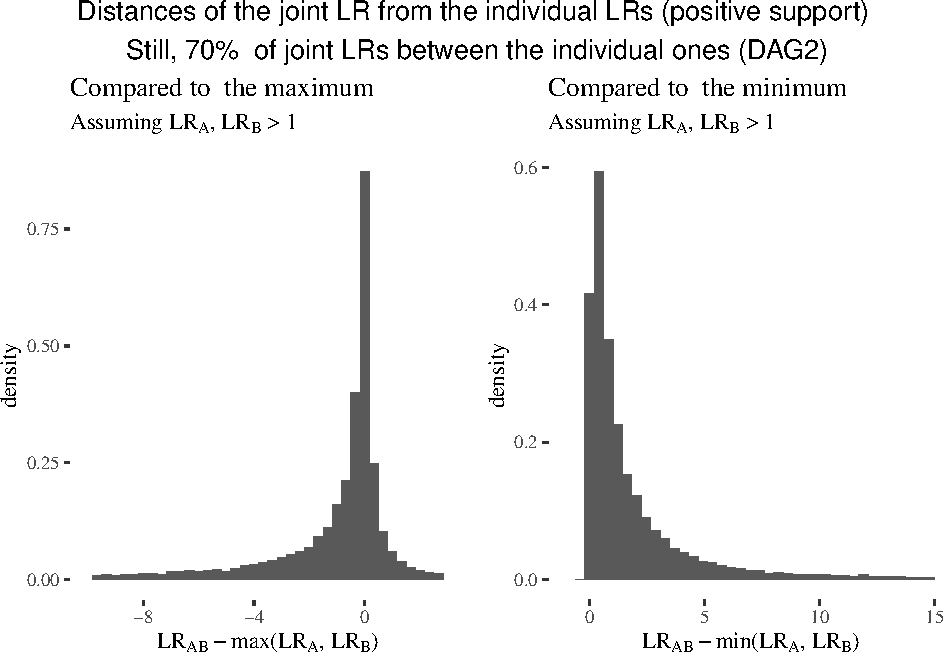
\includegraphics[width=0.7\linewidth]{conjunction-appendix14_files/figure-latex/unnamed-chunk-23-1} \end{center}

\caption{Distances of joint likelihood ratios for the minima and the maxima of the individual likelihood ratios if the individual likelihood ratios are above 1, DAG used in \textsf{DAG2}.}
\label{fig:LRabovePlotDep}
\end{figure}

\begin{figure}


\begin{center}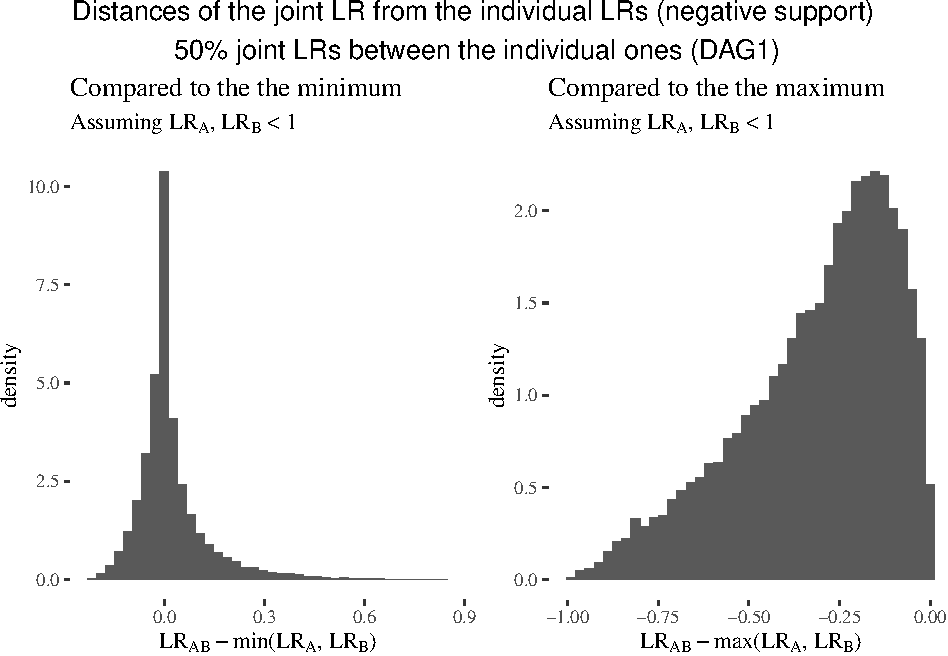
\includegraphics[width=0.7\linewidth]{conjunction-appendix14_files/figure-latex/unnamed-chunk-24-1} \end{center}

\caption{Distances of joint likelihood ratios for the minima and the maxima of the individual likelihood ratios if the individual likelihood ratios are below 1, DAG used in \textsf{DAG1}.} 
\label{fig:LRlowerPlot}
\end{figure}

\begin{figure}


\begin{center}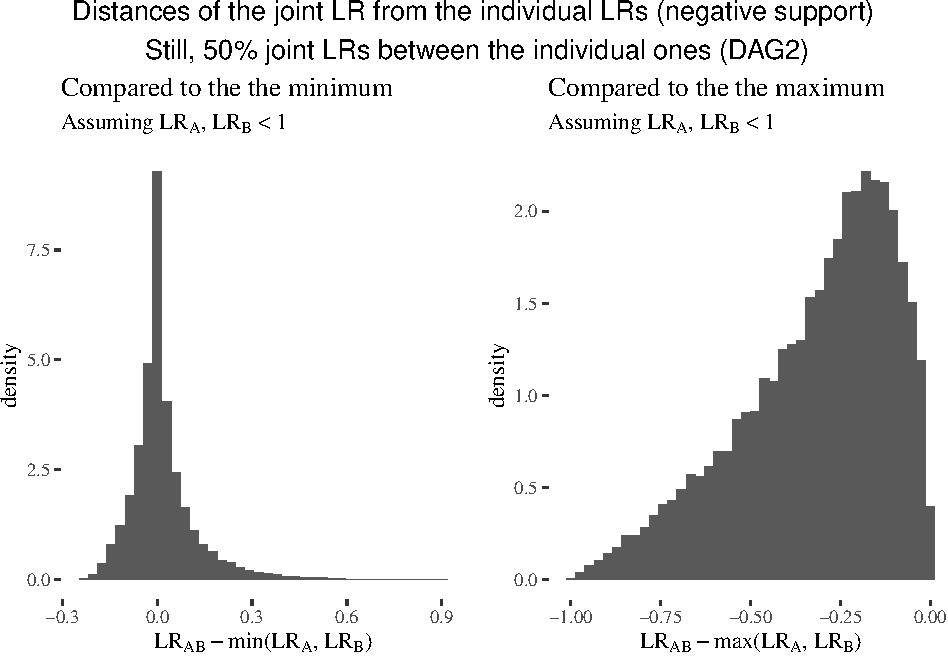
\includegraphics[width=0.7\linewidth]{conjunction-appendix14_files/figure-latex/unnamed-chunk-25-1} \end{center}

\caption{Distances of joint likelihood ratios for the minima and the maxima of the individual likelihood ratios if the individual likelihood ratios are below 1, DAG used in \textsf{DAG2}.} 
\label{fig:LRlowerPlot2}
\end{figure}

\newpage

These simulations demonstrate that, whenever individual \(LR_A\) and
\(LR_B\) are above a fixed threshold, so is the combined \(LR_{AB}\).
This fact justifies the principle of aggregation, as explained in the
main text of the chapter. The converse does not hold. Even when
\(LR_{AB}\) is above a threshold, \(LR_A\) or \(LR_B\) may be below the
threshold. Hence, as with the Bayes factor, the principle of
distribution fails in some cases.

\hypertarget{keeping-evidence-fixed}{%
\subsection*{Keeping evidence fixed}\label{keeping-evidence-fixed}}
\addcontentsline{toc}{subsection}{Keeping evidence fixed}

Recall the distinction between the two variants of the distribution
principle:

\begin{align}
S[a \wedge b, A\wedge B] \Rightarrow S[a, A] \wedge S[b, B] \tag{DIS1} \\
S[a \wedge b, A\wedge B] \Rightarrow S[a \wedge b, A] \wedge S[a\wedge b, B] \tag{DIS2}
\end{align}

\noindent \(S\) is a placeholder for the standard of proof. The
difference is whether or not the body of evidence is held constant. The
failures of distributions considered so far were failures of (DIS1).
Even when the combined Bayes factor or likelihood ratio meet a fixed
threshold, the individual measures may not. One wonders whether (DIS2)
could be easier to justify. To this end, consider:

\begin{align*}
LR_A^{ab}  & =  \frac{\pr{a \wedge b \vert A}}{\pr{a \wedge b}}\\
LR_B^{ab} & = \frac{\pr{a \wedge b \vert B}}{\pr{a \wedge b}}\\\
LR_{AB}^{ab}  & =  \frac{\pr{a\wedge b \vert A \wedge B}}{\pr{a \wedge b}}
\end{align*}

\noindent Note that the evidence \(a\wedge b\) is now held constant
across cases. A computer simulation shows that, even when
\(LR_{AB}^{ab}\) meets a fixed threshold, the individual \(LR_A^{ab}\)
and \(LR_B^{ab}\) may not. For \textsf{DAG1}, the joint likelihood ratio
\(LR_{AB}^{ab}\) is strictly greater than both of the individual
likelihood ratio \(LR_{A}^{ab}\) and \(LR_{B}^{ab}\) in 30\% of the
cases (22\% for \textsf{DAG2}). A similar conclusion holds for the Bayes
factor. So keeping the evidence fixed does not make it any easier to
justify distribution.\footnote{We run a number of computer simulations.
  For the sake of completeness, here are the results. If no assumption
  about the direction of support is made, around 12.7\% of the time
  (twice less often than if the usual individual likelihood ratio are
  used), the individual \(LR_A^{ab}\) and \(LR_B^{ab}\) are both greater
  than the joint \(LR_{AB}^{ab}\). This holds for \textsf{DAG1}. The
  frequency goes slightly up to around 13\% if we switch to
  \textsf{DAG2}. Assuming the individual likelihood ratios are above
  one, only about 70\% of joint likelihood ratios are between the
  individual ones in \textsf{DAG1} (75\% for \textsf{DAG2}) . However,
  no joint likelihood ratio is below the minimum of the individual
  ratios for \textsf{DAG1}, as expected. Interestingly, the join
  likelihood ratio may go below the minimum of the individual ones in
  very rare cases, 2\% of the times, for \textsf{DAG2}. . So, strictly
  speaking, aggregation can fail if dependencies are present so long as
  the evidence is held constant.}

\hypertarget{dependent-evidence}{%
\subsection*{Dependent evidence}\label{dependent-evidence}}
\addcontentsline{toc}{subsection}{Dependent evidence}

\textsf{DAG 1} and \textsf{DAG 2} ensure that the items of evidence are
conditionally independent on their respective hypothesis (specifically,
that \(a\) is independent both conditional on \(A\) and conditional on
\(\n A\), and the same for \(b\) and \(B\).).\footnote{In fact,
  \textsf{DAG 1} ensure that they are also unconditionally independent.}
The results established so far, then, rests on this assumption. What
happens if this independence is dropped? To investigate this question,
we run a simulation based on \textsf{DAG 3}, illustrated in Figure
\ref{fig:dag3}. As it turns out, the joint likelihood ratio can be lower
than both individual likelihood ratios and the joint Bayes factor lower
than both individual Bayes factors in 14\% cases. Crucially, this occurs
when the individual Bayes factor and likelihood ratios are greater than
one. An example is given in Figure \ref{fig:CPTDoubleL}. This result is,
of course, nothing surprising if we keep in mind that, in
\textsf{DAG 3}, the items of evidence no longer count as independent
lines of evidence.

\vspace{1mm}
\footnotesize

\normalsize

\begin{figure}[H]


\begin{center}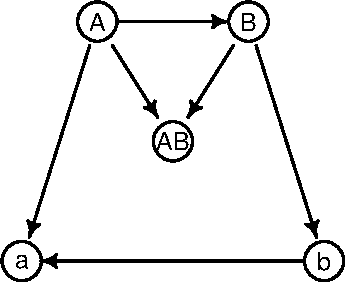
\includegraphics[width=0.7\linewidth]{conjunction-appendix14_files/figure-latex/unnamed-chunk-27-1} \end{center}
\caption{\textsf{DAG 3} with direct dependence between the pieces of evidence.}
\label{fig:dag3}
\end{figure}

\begin{figure}
\hspace{2mm}\begin{subfigure}[ht!]{0.45\textwidth}
\footnotesize


\begin{tabular}{lr}
\toprule
A & Pr\\
\midrule
\cellcolor{gray!6}{1} & \cellcolor{gray!6}{0.521}\\
0 & 0.479\\
\bottomrule
\end{tabular}

\vspace{2mm}

\begin{tabular}{lrr}
\toprule
\multicolumn{1}{c}{B} & \multicolumn{2}{c}{A} \\
  & 1 & 0\\
\midrule
\cellcolor{gray!6}{1} & \cellcolor{gray!6}{0.66} & \cellcolor{gray!6}{0.729}\\
0 & 0.34 & 0.271\\
\bottomrule
\end{tabular}

\vspace{2mm}

\begin{tabular}{lllr}
\toprule
\multicolumn{1}{c}{} & \multicolumn{1}{c}{A} & \multicolumn{1}{c}{b} & \multicolumn{1}{c}{} \\
a &  &  & Pr\\
\midrule
\cellcolor{gray!6}{1} & \cellcolor{gray!6}{1} & \cellcolor{gray!6}{1} & \cellcolor{gray!6}{0.3989398}\\
0 & 1 & 1 & 0.6010602\\
\cellcolor{gray!6}{1} & \cellcolor{gray!6}{0} & \cellcolor{gray!6}{1} & \cellcolor{gray!6}{0.9673984}\\
0 & 0 & 1 & 0.0326016\\
\cellcolor{gray!6}{1} & \cellcolor{gray!6}{1} & \cellcolor{gray!6}{0} & \cellcolor{gray!6}{0.9693564}\\
0 & 1 & 0 & 0.0306436\\
\cellcolor{gray!6}{1} & \cellcolor{gray!6}{0} & \cellcolor{gray!6}{0} & \cellcolor{gray!6}{0.7267025}\\
0 & 0 & 0 & 0.2732975\\
\bottomrule
\end{tabular}

\vspace{2mm}

\begin{tabular}{lrr}
\toprule
\multicolumn{1}{c}{b} & \multicolumn{2}{c}{B} \\
  & 1 & 0\\
\midrule
\cellcolor{gray!6}{1} & \cellcolor{gray!6}{0.995} & \cellcolor{gray!6}{0.108}\\
0 & 0.005 & 0.892\\
\bottomrule
\end{tabular}

\normalsize 


\subcaption{Conditional probabilities for the counterexample (the one for \textsf{AB} does not change).}
\end{subfigure} 
\hspace{5mm}\begin{subfigure}{0.45\textwidth}

\begin{center}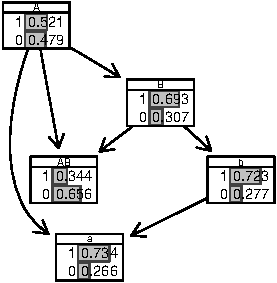
\includegraphics[width=0.7\linewidth]{conjunction-appendix14_files/figure-latex/unnamed-chunk-29-1} \end{center}
\subcaption{Marginal probabilities. }
\end{subfigure} 
\caption{A counterexample based on \textsf{DAG 3}, with independence between the items of evidence dropped.   $LR_A  \approx 1.063$, $LR_B \approx 1.159742$,  $LR_{AB} \approx 0.651$. $BF_A \approx  1.022, BF_B \approx  1.079, BF_{AB}\approx   0.699$.}
\label{fig:CPTDoubleL}
\end{figure}

.

\end{document}
